\section{Performance Evaluation}
Now, if everything is correctly done and the configUSE\_RM value is equal to 1, the RM scheduler can be tested.\\
The same benchmark was adapted to be tested with the two different scheduling algorithms (default FreeRTOS scheduling algorithm and RM scheduling). The benchmark creates three tasks that occupy the CPU for a specific time. After execution, the tasks release the CPU and are recreated after a certain period of time. In both tests, the tasks had the same priority, but in the RM-related benchmark, they had different periods and burst times. The two benchmarks generate output to text files, which are then used to generate a graph and compare the statistics of the two scheduling algorithms.

\begin{figure}[H]
    \centering
    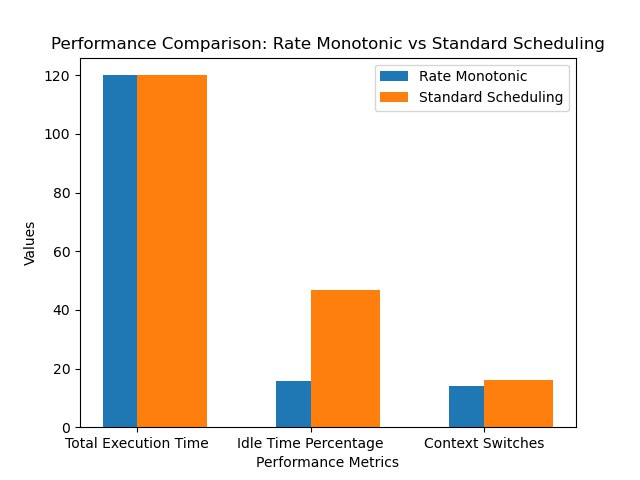
\includegraphics[width=1\linewidth]{img/performance.jpg}
    \caption{Performance Evaluation Comparison (RM Scheduling and Default FreeRTOS Scheduling Algorithm)}
    \label{fig:performance}
\end{figure}

The image shows:
\begin{itemize}
    \item \textbf{Total Execution Time}:
    \begin{itemize}
        \item Both the Rate Monotonic scheduler and the standard FreeRTOS scheduler are executed for 120 seconds.
    \end{itemize}
    \item \textbf{Idle Time Percentage}:
    \begin{itemize}
        \item The standard FreeRTOS scheduler shows a significantly higher idle time percentage compared to the Rate Monotonic scheduler.
        \item This indicates that the RM algorithm is more efficient in utilizing CPU time, reducing the periods when the CPU remains idle.
    \end{itemize}
    \item \textbf{Context Switches}:
    \begin{itemize}
        \item The standard FreeRTOS scheduler has a slightly higher number of context switches compared to the Rate Monotonic scheduler.
        \item Context switches represent the operating system's overhead, so a lower number of context switches in the RM case suggests greater efficiency.
    \end{itemize}
\end{itemize}

\noindent The FreeRTOS scheduler exhibits more idle time because, when tasks have the same priority, FreeRTOS allows multiple tasks to run in parallel (multitasking). This can be both an advantage and a disadvantage when a task is waiting for data from other tasks. Additionally, the context switches are higher in the default FreeRTOS scheduling because multitasking implies that tasks are repeatedly switched after having a common CPU time slice.